% !TEX encoding = UTF-8 Unicode
\documentclass[a4paper]{article}

\usepackage{lipsum}
\usepackage{tcolorbox}
\usepackage{color}
\usepackage{url}
%\usepackage[T2A]{fontenc} % enable Cyrillic fonts
\usepackage[utf8]{inputenc} % make weird characters work
\usepackage{graphicx}
\usepackage{amsmath}
%\usepackage[obeyspaces]{url}
\usepackage[T1]{fontenc}
% \usepackage{inconsolata}

\usepackage[english,serbian]{babel}
%\usepackage[english,serbianc]{babel} %ukljuciti babel sa ovim opcijama, umesto gornjim, ukoliko se koristi cirilica

\usepackage[german=quotes]{csquotes}
\DeclareQuoteAlias{ngerman}{serbian}
\MakeOuterQuote{"}

\usepackage[unicode]{hyperref}
\hypersetup{colorlinks,citecolor=green,filecolor=green,linkcolor=blue,urlcolor=blue}

\usepackage{epigraph}

\usepackage{listings}

%\newtheorem{primer}{Пример}[section] %ćirilični primer
\newtheorem{primer}{Primer}[section]

\definecolor{mygreen}{rgb}{0,0.6,0}
\definecolor{mygray}{rgb}{0.5,0.5,0.5}
\definecolor{mymauve}{rgb}{0.58,0,0.82}


\lstset{ 
  backgroundcolor=\color{white},   % choose the background color; you must add \usepackage{color} or \usepackage{xcolor}; should come as last argument
  basicstyle=\scriptsize\ttfamily,        % the size of the fonts that are used for the code
  breakatwhitespace=false,         % sets if automatic breaks should only happen at whitespace
  breaklines=true,                 % sets automatic line breaking
  captionpos=b,                    % sets the caption-position to bottom
  commentstyle=\color{mygreen},    % comment style
  deletekeywords={...},            % if you want to delete keywords from the given language
  escapeinside={\%*}{*)},          % if you want to add LaTeX within your code
  extendedchars=true,              % lets you use non-ASCII characters; for 8-bits encodings only, does not work with UTF-8
  firstnumber=1000,                % start line enumeration with line 1000
  frame=single,	                   % adds a frame around the code
  keepspaces=true,                 % keeps spaces in text, useful for keeping indentation of code (possibly needs columns=flexible)
  keywordstyle=\color{blue},       % keyword style
  language=Python,                 % the language of the code
  morekeywords={*,...},            % if you want to add more keywords to the set
  numbers=left,                    % where to put the line-numbers; possible values are (none, left, right)
  numbersep=5pt,                   % how far the line-numbers are from the code
  numberstyle=\tiny\color{mygray}, % the style that is used for the line-numbers
  rulecolor=\color{black},         % if not set, the frame-color may be changed on line-breaks within not-black text (e.g. comments (green here))
  showspaces=false,                % show spaces everywhere adding particular underscores; it overrides 'showstringspaces'
  showstringspaces=false,          % underline spaces within strings only
  showtabs=false,                  % show tabs within strings adding particular underscores
  stepnumber=2,                    % the step between two line-numbers. If it's 1, each line will be numbered
  stringstyle=\color{mymauve},     % string literal style
  tabsize=2,	                   % sets default tabsize to 2 spaces
  title=\lstname                   % show the filename of files included with \lstinputlisting; also try caption instead of title
}

\begin{document}

\title{Prepoznavanje vrste kancera metodom klasifikacije\\ \small{Seminarski rad u okviru kursa\\Istraživanje podataka\\ Matematički fakultet, Univerzitet u Beogradu}}

\author{Nadežda Bogdanović\\1093/2018\\\small{nadezdabogdanovic1@gmail.com}}

\date{19.06.2019}

\maketitle

\abstract{
Cilj ovog rada je da potvrdi da li je moguće na osnovu podataka o mutiraim genima utvrditi koji je organ oboleo. Prilikom odgovora na ovo pitanje korišćene su različite metode klasifikacije obrađene u programskom jeziku Python, ili IBM-ovom alatu SPSS Modeler.
}


\newpage

\tableofcontents

\newpage


\section{Uvod}
\label{sec:Uvod}

Kada zdrava ćelija postane kancerogena, dese se  promene u njenom genetskom materijalu - on se izmeni. Postavlja se pitanje: Da li je moguće utvrditi koje tkivo je kontaminirano na osnovu podataka dobijenih sekvenciranjem i upoređivanja sa referentnim genomom? Ovo istraživanje daje odgovor na takvo pitanje.

U drugom poglavlju čitalac se može upoznati sa podacima\cite{podaci}, koji su dobijeni kao rezultat rada alata ABSOLUTE\cite{ABSOLUTE}. Ovaj alat obrađuje podatke dobijene sekvenciranjem kancerogenih tkiva, upoređuje ih sa referentnim genomom i broji duplikacije i delecije koje su se desile u kontaminiranom genomu.

Primena klasifikacije na sirove podatke nije moguća. Treće poglavlje objašnjava kako je potrebno obraditi podatke, kako bi se dobili što bolji rezultati.

Četvrto, peto, šesto sedmo i osmo poglavlje upoređuju rezultate primenom različitih algoritama klasifikacije (drveta odlučivanja, najbliži susedi, neuronske mreže, potporni vektori i Gausova klasifikacija), obrađivanih u programskom jeziku Python, ili u SPSS Modeleru. Kodovi koji su predstavljeni u ovom radu preuzeti su sajta asistenta ovog predmeta\cite{mm}, Mirjane Maljković, i izmenjeni u skladu sa potrebom.

\newpage

\section{Upoznavanje sa podacima}
\label{sec:Upoznavanje}

Podaci se mogu pronaći na \url{https://portals.broadinstitute.org/ccle/data} pod nazivom \textbf{CCLE\_ABSOLUTE\_combined 20181227.xlsx}. U okviru fajla postoje 3 lista:
\begin{itemize}
    \item \textbf{ABSOLUTE\_combined.segtab} - sadrži podatke nad kojima se vrši istraživanje: 20 kolona i 188653 redova
    \item \textbf{segtab annotations} - sadrži objašnjenje naziva atribta sa prvog lista
    \begin{itemize}
        \item Sample: naziv ćelijske linije sa koje je uzet uzorak. Sastoji se od naziva tkiva koje je sekvencirano i jedinstvenog identifikatora.
        \item Chromosome: hromozom na kojem se nalazi mutirani segment.
        \item Start: početna pozicija mutiranog segmenta na datom hromozomu.
        \item End: krajnja pozicija mutiranog segmenta na datom hromozomu.
        \item Num\_Probes: broj SNP satelita (sateliti su markeri koji se koriste prilikom sekvencirnja) na datom segnemtu\cite{SNP}.
        \item Length : Dužina mutiranog segmenta.
        \item Modal\_HSCN\_1: broj apsolutnih duplikacija/delecija na alternativnom alelu.
        \item Modal\_HSCN\_2: broj apsolutnih duplikacija/delecija na referentnom alelu.
        \item Modal\_HSCN\_TOTAL:  Modal\_HSCN\_1 +  Modal\_HSCN\_2. 
        \item Subclonal\_HSCN\_a1: broj apsolutnih duplikacija/delecija na alternativnom alelu u subklonalnoj populaciji (populacija mutiranih kancerogenih ćelija koja je mutirala od početne kancerogene ćelije)\cite{subclonal}.
        \item Subclonal\_HSCN\_a1: broj apsolutnih duplikacija/delecija na referentnom alelu u subklonalnoj populaciji.
        \item Cancer\_cell\_frac\_a1: maksimalna procena za udeo ćelija koje nose mutaciju na prvom alelu.
        \item Ccf\_ci95\_low\_a1: donja granica 95\% intervala poverenja za udeo ćelija koje nose mutaciju na prvom alelu.
        \item Ccf\_ci95\_high\_a1: gornja granica 95\% intervala poverenja za udeo ćelija koje nose mutaciju na prvom alelu.
        \item ancer\_cell\_frac\_a2: maksimalna procena za udeo ćelija koje nose mutaciju na drugom alelu.
        \item Ccf\_ci95\_low\_a2: donja granica 95\% intervala poverenja za udeo ćelija koje nose mutaciju na drugom alelu.
        \item Ccf\_ci95\_high\_a2: gornja granica 95\% intervala poverenja za udeo ćelija koje nose mutaciju na drugom alelu.
        \item LOH: gubitak heterozigosnosti na datom segmentu.
        \item Homozygos\_deletion: oznaka da li je dati segment homozigotno obrisan ili ne.
        \item depMapID: jedinstveni ID uzorka, koji se koristi za povezivanje sa drugim fajlovima.
    \end{itemize}
    \item \textbf{ABSOLUTE\_combined.table}: sadrži opise podataka sa prvog lista
\end{itemize}.

\section{Priprema podataka za obradu}
\label{sec:preprocesiranje}

Ako se algoritam drveta odlučivanja pisanog u programskom jeziku Python primeni na neobrađene podatke, pogađanje klase odvija se sa preciznošću od 0,5\%. To se dešava iz nekoliko razloga koji će u daljem tekstu biti razmotreni.

\subsection{Problem prevelikog broja klasa}
\label{subsec:brojklasa}

Kada pokušamo da odredimo koje su sve moguće klase, videćemo da se u koloni \textit{Sample} nalazi 999 različitih vrednosti, samim tim i 999 različitih klasa. To je zato što se vrednosti u ovoj koloni sastoje od naziva tkiva koje je sekvencirano i jedinstvenog identifikatora. Kako nas zanima samo koji je organ oboleo, neophodno je grupisati sve podatke iz istog tkiva.

Koristeći SPSS Modeler i čvor \textit{Split} (fajl \textit{find\_most\_frequent.str}), možemo izdvojiti tkiva po uslovu \textit{hassubstring}, što nam daje 24 različite klase sa brojem instanci koje im pripadaju:
\begin{itemize}
    \item LUNG: 38,882
    \item SALIVARY\_GLAND: 358
    \item FIBROBLAST: 1,164
    \item PLEURA: 1,529
    \item THYROID: 2,824
    \item PANCREAS: 6,943
    \item BONE: 3,579
    \item STOMACH: 8,720
    \item UPPER\_AERODIGESTIVE: 5,970
    \item BREAST: 15,488
    \item CENTRAL\_NERVOUS\_SYSTEM: 12,357
    \item PROSTATE: 1,356
    \item INTESTINE: 9,369
    \item SOFT\_TISSUE: 3,475
    \item ENDOMETRIUM: 5,277
    \item AUTNOMIC\_GANGLIA: 2,115
    \item HAEMATOPOIETIC\_AND\_LYMPHOID\_TISSUE: 27,115
    \item KIDNEY: 4,171
    \item BILIARY\_TRACT: 1,462
    \item OESOPHAGUS: 7,798
    \item OVARY: 11,584
    \item URINARY\_TRACT: 4,073
    \item LIVER: 4,718
    \item SKIN: 8,384
\end{itemize}

Ako algoritam primenimo sada, dobićemo preciznosti od 5\%. To nas dovodi do zaključka da je nedovoljan broj instanci po klasi, što znači da ćemo najpreciznija pogađanja dobiti ako odaberemo da radimo samo s klasama sa najvećim brojem instanci: LUNG i HAEMATOPOIETIC\_AND LYMPHOID\_TISSUE. Koristeći čvor \textit{Append} (fajl \textit{MERGE.str}), objedinićemo podatke sa oznakama ove dve klase u poseban \textit{EXTRACTED CLASSES.xlsx} fajl. Međutim, on i dalje sadrži različite oznake za ista tkiva, tako da ćemo sve one koji sadrže podstring \textit{LU} predstaviti kao \textit{LUNG}, a one koji sadrže \textit{HA}, predstaviti kao \textit{HAEMATOPOIETIC} (fajl \textit{create\_finals.py}) i sačuvati u fajlu \textit{final\_X.xlsx} sa kojim ćemo nadalje raditi, gde umesto X može stajati implicit ili explicit, što zavisi od korišćene metode objašnjene u poglavlju \ref{subsec:geni}.

\lstinputlisting[language=Python, caption={Prečišćavanje klasa},frame=single, label=classes]{classes.py}

Dobijene klase predstavljene su na slici \ref{fig:classes2}:
\begin{figure}[ht!]
                \centering
                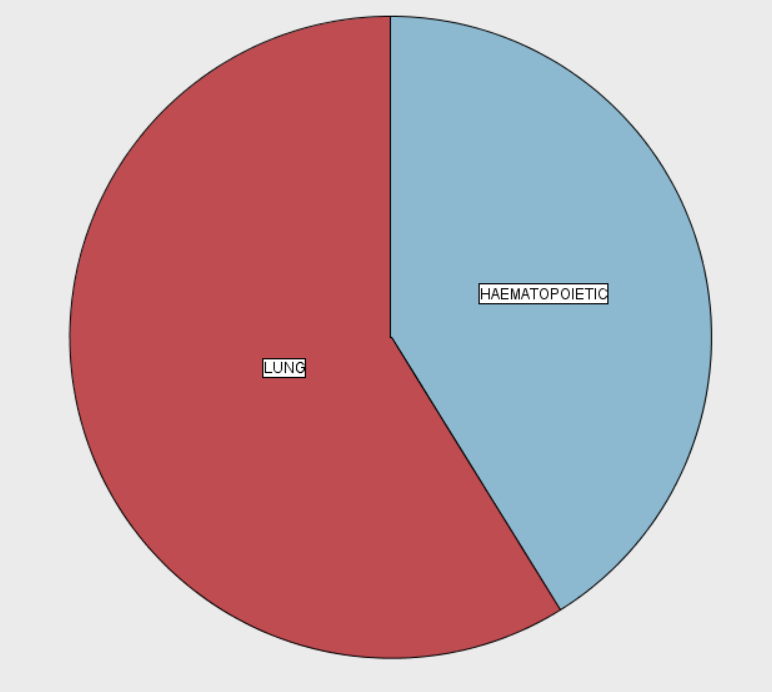
\includegraphics[width=0.5\textwidth]{classes_2.PNG}
                \caption{Klase}
                \label{fig:classes2}
            \end{figure}


\subsection{Problem nedostajućih vrednosti}
\label{subsec:nedostajuce}

Pre nego što spojimo željene klase u odgovarajući fajl, proverićemo da li postoje nedostajuće vrednosti, ili elementi van granica. Ako pokrenemo čvor \textit{Data Audit} i u njemu otvorimo karticu \textit{Quality}, videćemo da su podaci 98.47\% kompletni. Sa nedostajućim vrednostima se nosimo tako što generišemo super čvor u kojem nedostajuće vrednosti zamenjujemo srednjim vrednostima.

Atributi Start, End, Num\_Probes, Length, Modal\_HSCN\_1 i Modal\_HSCN\_2 sadrže ekstremne vrednosti i vrednosti van granica. Sa atributima Start, End i Num\_Probes ćemo se pozabaviti u odeljku \ref{subsec:geni}, a sa Length, Modal\_HSCN\_1 i Modal\_HSCN\_2 u odeljku \ref{subsec:korelacija}.

\subsection{Problem definisanja mutiranih gena}
\label{subsec:geni}

Kao što je već rečeno, pokušavamo da dokažemo da na osnovu mutiranih (grupa) gena možemo da odredimo koje tkivo je obolelo. Iako u ovim podacima ne nalazimo eksplicitne oznake gena, ipak ih možemo razlikovati na osnovu njihove lokacije koja je sačinjena od početka i kraja mutiranog segmenta koji se nalaze na određenom hromozomu. Međutim, razlika između najmanjih i najvećih vrednosti u ovim atributima, kao i u Num\_Probes je tako velika (24,9087,712 za Start, 249,133,375 za End i 72,607 za Num\_Probes), da ih je teško pratiti, a pored toga, javljaju se i ekstremne vrednosti i elementi van granica. Postoje 2 načina da se ovaj problem reši i ovo istraživanje će ispratiti oba:
\begin{enumerate}
    \item Implicitno definianje: Koristeći SPSS Modelerov čvor \textit{Binning}, vrednostima gorenavedenih atributa su dodeljene oznake brojevnih opsega kojima pripadaju, kao što je prikazano na slici \ref{fig:classes}. Vrednosti se grupišu tako da u svakoj grupi bude jednak broj vrednosti (\textit{TILES}) po decilima.
    
    \begin{figure}[ht!]
                \centering
                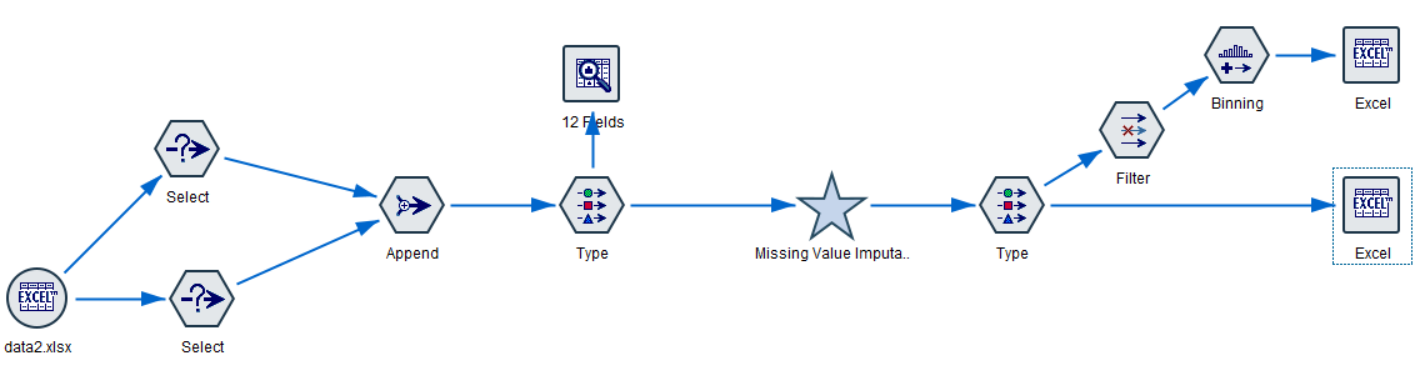
\includegraphics[width=0.9\textwidth]{classes.PNG}
                \caption{Implicitan i eksplicitan način}
                \label{fig:classes}
            \end{figure}
    
    \item Eksplicitno definisanje gena: Podaci se u SPSS Modeleru pomoću čvora \textit{Split} razvrstaju po hromozomima i čuvaju u posebnim fajlovima (\textit{chromosome\_pp.str}). Zatim se, kao što je prikazano na kodu, svakoj instanci dodeljuju oznake genskih grupa koje su zahvaćene mutacijom (\textit{Genes.py}). Nakon toga se  obrađeni fajlovi objedinjuju u jedan (\textit{EXCTRACTED\_CLASSES\_chromosome.xlsx}) pomoću čvora \textit{Append} u SPSS Modeleru (\textit{merge\_chromosome.str}). Konačno, na taj fajl se primeni već prikazani algoritam prečišćavanja vrednosti atributa \textit{sample}.
    
    \lstinputlisting[language=Python, caption={Definisanje klasa},frame=single, label=classes]{chromosomes.py}
\end{enumerate}

\subsection{Problem korelisanih atributa}
\label{subsec:korelacija}

Pozivanjem \textit{dataframe.corr()['atribut']} u programskom jeziku Python nad skupom podataka, izračunate su sledeće stope korelacije i prikazane u tabelama \ref{tab:korelacije1}, \ref{tab:korelacije2}, \ref{tab:korelacije3}, \ref{tab:korelacije4}, \ref{tab:korelacije5}:

\begin{table}[ht!]
\begin{center}
\caption{Korelacija između atributa}
\label{tab:korelacije1}
\begin{tabular}{c|c|c|c|c} \hline
& \textbf{Chromosome} & \textbf{Start} & \textbf{End} & \textbf{Gene}\\ \hline
\textbf{Chromosome} & 1.0 & x & x & 0.99 \\ \hline
\textbf{Start} & x & 1.0 & 0.93 & x\\ \hline
\textbf{End} & x & 0.93 & 1.0 & x\\ \hline
\textbf{Gene} & 0.99 & x & x & 1.0\\ \hline
\end{tabular}
\end{center}
\end{table}

\begin{table}[ht!]
\begin{center}
\caption{Korelacija između atributa}
\label{tab:korelacije2}
\begin{tabular}{c|c|c|c|c} \hline
& \textbf{Sample} & \textbf{Num Probes} & \textbf{Length} & \textbf{depMapID}\\ \hline
\textbf{Sample} & 1.0 & x & x & 1.0 \\ \hline
\textbf{Num Probes} & x & 1.0 & 0.98 & x \\ \hline
\textbf{Length} & x & 0.98 & 1.0 & x\\ \hline
\textbf{depMapID} & 1.0 & x & x & 1.0 \\ \hline
\end{tabular}
\end{center}
\end{table}

\begin{table}[ht!]
\begin{center}
\caption{Korelacija između atributa}
\label{tab:korelacije3}
\begin{tabular}{c|c|c|c|c} \hline
& \textbf{Modal 1} & \textbf{Modal 2} & \textbf{Modal Total} & \textbf{LOH}\\ \hline
\textbf{Modal 1} & 1.0 & x & x & -0.82\\ \hline
\textbf{Modal 2} & x & 1.0 & 0.88 & x\\ \hline
\textbf{Modal Total} & x & 0.88 & 1.0 & x\\ \hline
\textbf{LOH} & -0.82 & x & x & 1.0\\ \hline
\end{tabular}
\end{center}
\end{table}



\begin{table}[ht!]
\begin{center}
\caption{Korelacija između atributa}
\label{tab:korelacije4}
\begin{tabular}{c|c|c|c} \hline
& \textbf{Cancer Frac a1} & \textbf{Ccf low a1} & \textbf{Ccf high a1} \\ \hline
\textbf{Cancer Frac a1} & 1.0 & 0.97 & 0.98\\ \hline
\textbf{Ccf low a1} & 0.97 & 1.0 & 0.94\\ \hline
\textbf{Ccf high a1} & 0.98 & 0.94 & 1.0\\ \hline
\end{tabular}
\end{center}
\end{table}

\begin{figure}[ht!]
                \centering
                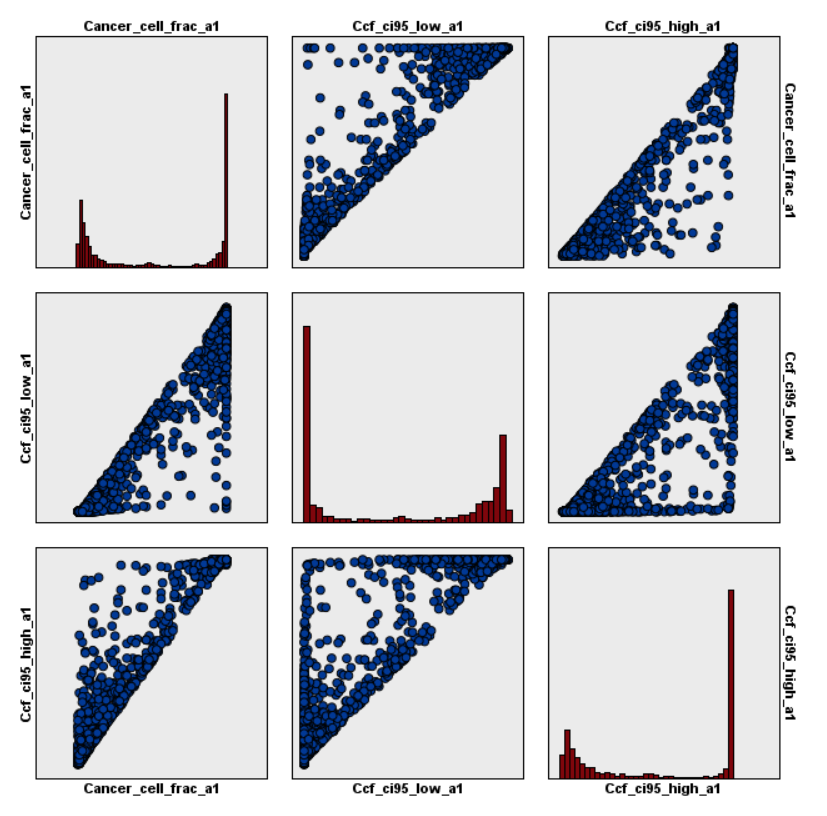
\includegraphics[width=0.9\textwidth]{korel_frac.PNG}
                \caption{Korelacija atributa Cancer\_Frac\_a1, Ccf\_low\_a1, Ccf\_high\_a1}
                \label{fig:korel_frac}
            \end{figure}

\begin{table}[ht!]
\begin{center}
\caption{Korelacija između atributa}
\label{tab:korelacije5}
\begin{tabular}{c|c|c|c} \hline
& \textbf{Cancer Frac a2} & \textbf{Ccf low a2} & \textbf{Ccf high a2} \\ \hline
\textbf{Cancer Frac a2} & 1.0 & 0.97 & 0.97\\ \hline
\textbf{Ccf low a2} & 0.97 & 1.0 & 0.92\\ \hline
\textbf{Ccf high a2} & 0.97 & 0.92 & 1.0\\ \hline
\end{tabular}
\end{center}
\end{table}

Za metodu koja koristi grupisanje postoje još i dodatne  korelacije prikazane u tabelama \ref{tab:korelacije6} i \ref{tab:korelacije7}:

\begin{table}[ht!]
\begin{center}
\caption{Korelacija između atributa}
\label{tab:korelacije6}
\begin{tabular}{c|c|c|c|c} \hline
& \textbf{Start} & \textbf{End} & \textbf{Start TILE10} & \textbf{End TILE10}\\ \hline
\textbf{Start} & 1.0 & 0.92 & 0.94 & 0.87\\ \hline
\textbf{End} & 0.92 & 1.0 & 0.86 & 0.95\\ \hline
\textbf{Start TILE10} & 0.94 & 0.86 & 1.0 & 0.89\\ \hline
\textbf{End TILE10} & 0.87 & 0.95 & 0.89 & 1.0\\ \hline
\end{tabular}
\end{center}
\end{table}

Ovo je grafički prikazano na slici \ref{fig:korel_se}.
\begin{figure}[ht!]
                \centering
                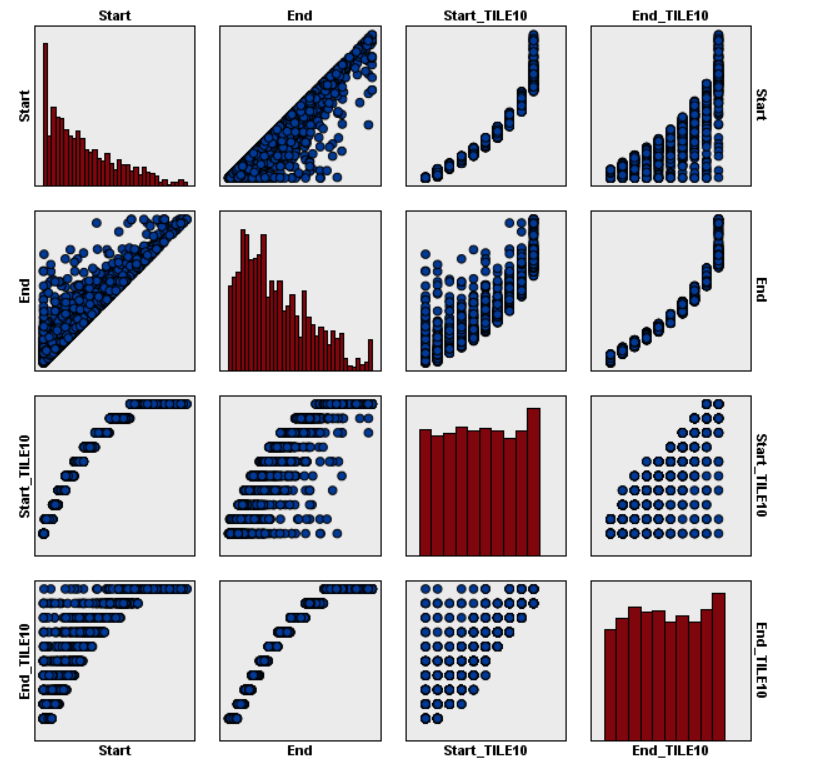
\includegraphics[width=0.9\textwidth]{korel_se.PNG}
                \caption{Korelacija atributa Start, End, Start\_TILE10 i End\_TILE10}
                \label{fig:korel_se}
            \end{figure}

\begin{table}[ht!]
\begin{center}
\caption{Korelacija između atributa}
\label{tab:korelacije7}
\begin{tabular}{c|c|c} \hline
& \textbf{Num Probes} & \textbf{Num Probes TILE10}\\ \hline
\textbf{Num Probes} & 1.0 & 0.75\\ \hline
\textbf{Num Probes TILE10} & 0.75 & 1.0\\ \hline
\end{tabular}
\end{center}
\end{table}

Ovo je grafički prikazano na slici \ref{fig:korel_num}.
\begin{figure}[ht!]
                \centering
                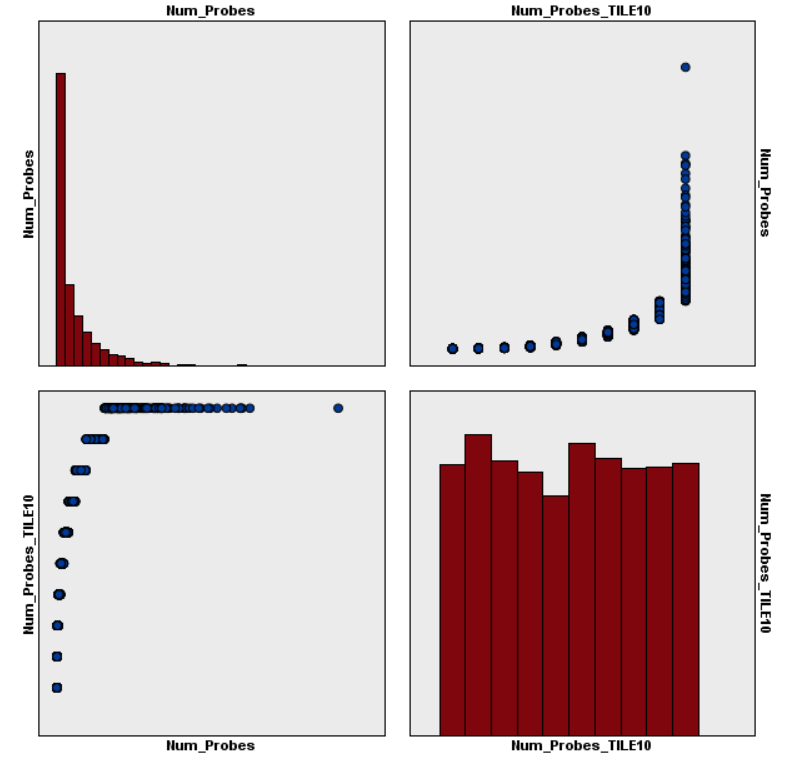
\includegraphics[width=0.9\textwidth]{korel_num.PNG}
                \caption{Korelacija atributa Num\_Probes i Num\_Probes\_TILE10}
                \label{fig:korel_num}
            \end{figure}

Na osnovu predloženog, odabrani su atributi koji će se koristiti za modeliranje: Start, Num Probes, Modal HSCn 1, Modal HSCN 2, Cancer cell frac a1, Cancer cell frac a2, Homozygos deletion, Gene; a za metodu koja koristi grupisanje Chromosome, Start TILE10, Num Probes TILE10, Modal HSCn 1, Modal HSCN 2, Cancer cell frac a1, Cancer cell frac a2, Homozygos deletion.


\section{Drveta odlučivanja}
\label{sec:drveta}

\subsection{SPSS Modeler}

U nastavku će biti upoređeni rezultati primene algoritama C5.0 (u fajlu \textit{C50.str}) i C\&R (u fajlu \textit{CRT.str}). U čvoru \textit{Partition} se vrši podela na traning, test i validacioni skup uzimajući 70\%, 20\% i 10\% podataka.

\subsubsection{C5.0}
\label{subsubsec:c50}

Čvor \textit{C.50} se spaja sa \textit{Partition} i to sa sledećeim opcijama: \textit{Group symbolics, Use boosting i Cross-validate}. Pokretanjem dobija se model koji analiziramo pomoću čvora \textit{Analyze}. Rezultati dobijeni implicitnim i eksplicitnim grupisanjem, mogu se uporediti na sledeći način:

            \begin{figure}[ht]
                \centering
                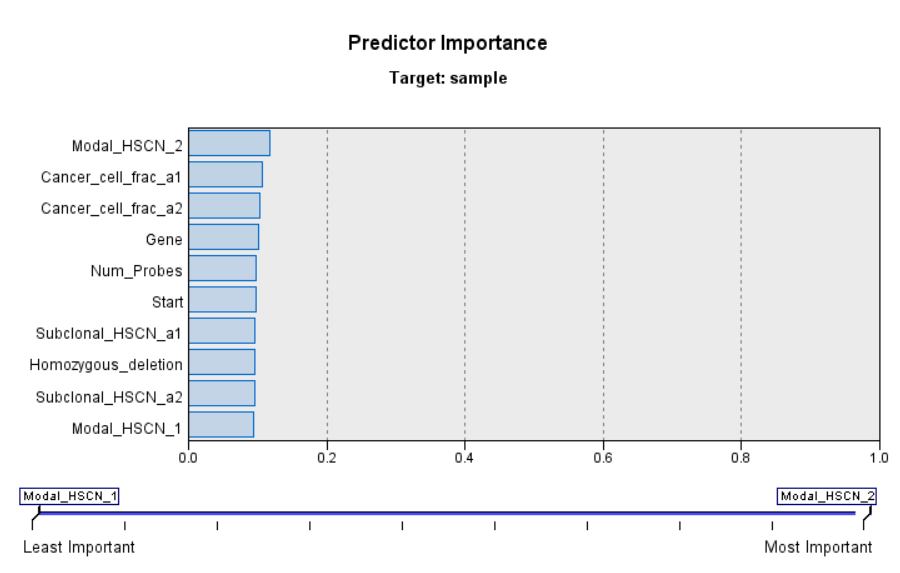
\includegraphics[width=0.7\textwidth]{C50_model_explicit.PNG}
                \caption{Bitnost atributa pri eksplicitnom grupisanju - C5.0}
                \label{fig:c50_predictor_ex}
            \end{figure}
            
            \begin{figure}[ht]
                \centering
                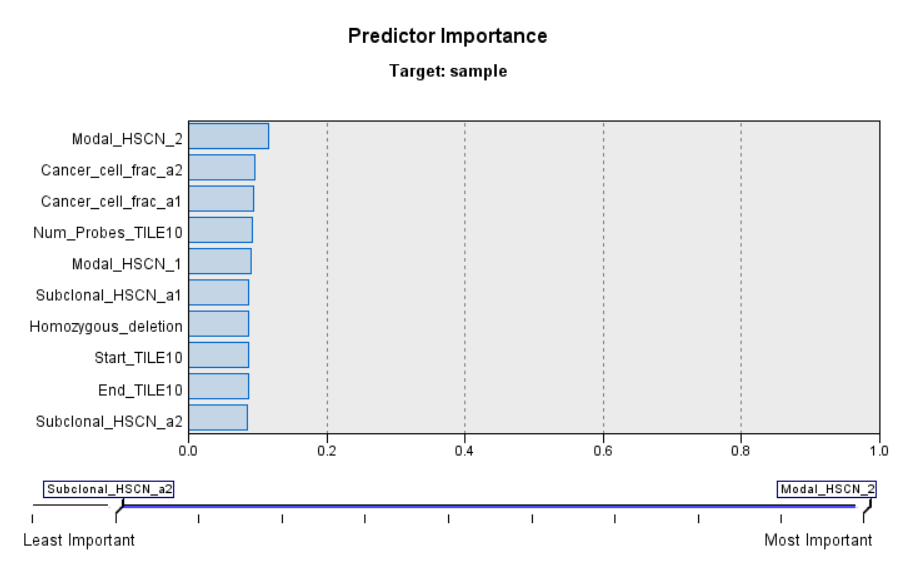
\includegraphics[width=0.7\textwidth]{C50_model_implicit.PNG}
                \caption{Bitnost atributa pri implicitnom grupisanju - C5.0}
                \label{fig:c50_predictor_im}
            \end{figure}

\begin{itemize}
    \item eksplicitno
        \begin{itemize}
            \item Dubina drveta: 17
            \item Standardna greška: 0.2
            \item Sredina: 65.2
            \item Najbitniji atribut za odlučivanje (slika \ref{fig:c50_predictor_ex}): Modal HSCN 2
            \item Najmanje bitan atribut za odlučivanje (slika \ref{fig:c50_predictor_ex}): Modal HSCN1
            \item preciznost je prikazana na slici \ref{fig:c50_analysis_ex}:
            \begin{figure}[ht]
                \centering
                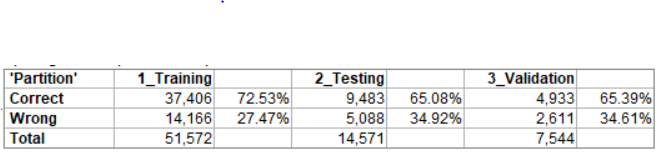
\includegraphics[width=0.7\textwidth]{C50_analysis_explicit.PNG}
                \caption{Analiza dobijenog modela pri eksplicitnom grupisanju - C5.0}
                \label{fig:c50_analysis_ex}
            \end{figure}
        \end{itemize}
    \item implicitno
    \begin{itemize}
        \item Dubina drveta: 23
        \item Sredina 70.5
            \item Standardna greška: 0.2
            \item Najbitniji atribut za odlučivanje (slika \ref{fig:c50_predictor_im}): Modal HSCN 2
            \item Najmanje bitan atribut za odlučivanje (slika \ref{fig:c50_predictor_im}): Subclonal HSCN a2
            \item preciznost je prikazana na slici \ref{fig:c50_analysis_im}:
            \begin{figure}[ht]
                \centering
                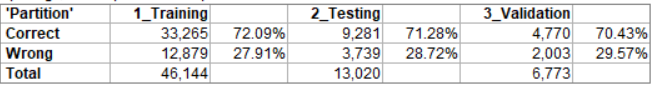
\includegraphics[width=0.7\textwidth]{C50_analysis_implicit.PNG}
                \caption{Analiza dobijenog modela pri implicitnom grupisanju - C5.0}
                \label{fig:c50_analysis_im}
            \end{figure}
    \end{itemize}
\end{itemize}

\subsubsection{C\&RT}
\label{subsubsec:CRT}

Model se pravi pomoću čvora \textit{C\&RT} nad \textit{final\_implicit.xlsx} podacima. Cilj je izgraditi novi model u vidu drveta odlučivanja maksimalne dubine 12. Minimalan broj instanci u grani roditelja je 5\%, a u grani deteta 2\%. Kao mera nečistoće koristi se Ginijev kriterijum i minimalnom promenom u nečistoći od 0.0001\%.

Analiza dobijenih rezultata može se videti na slici \ref{fig:crt_analysis}.

        \begin{figure}[ht!]
                \centering
                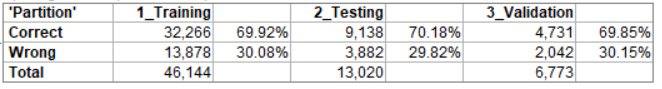
\includegraphics[width=0.9\textwidth]{CRT_analysis.PNG}
                \caption{Analiza drveta odlučivanja}
                \label{fig:crt_analysis}
            \end{figure}
            
Na slici \ref{fig:crt_tree} je prikazano drvo odlučivanja dobijeno generisanjem modela.
\begin{figure}[ht!]
                \centering
                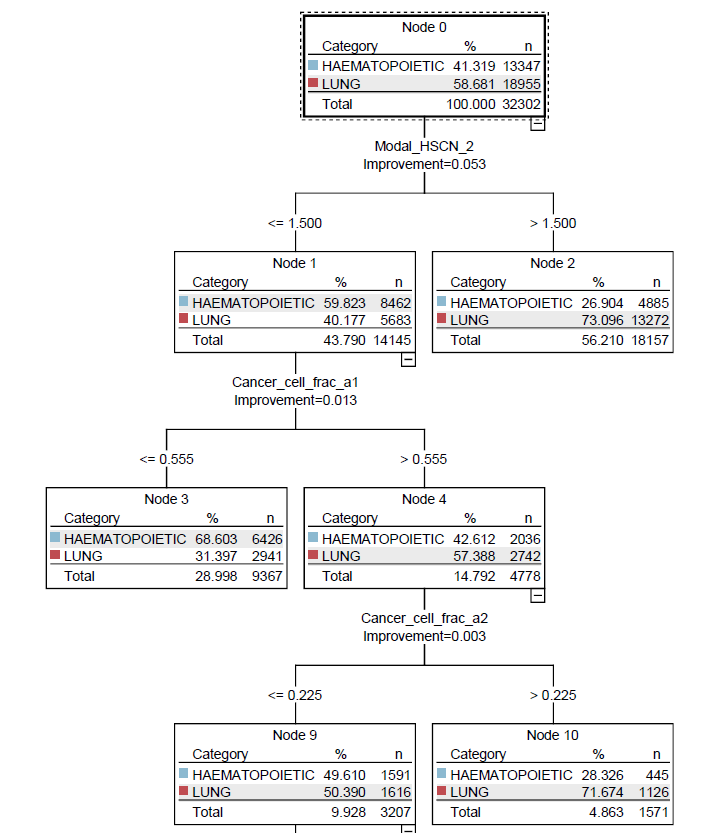
\includegraphics[width=0.9\textwidth]{CRT_model.PNG}
                \caption{Drvo odlučivanja - C\&RT}
                \label{fig:crt_tree}
            \end{figure}

\subsection{Python}

Primena algoritma drveta odlučivanja u programskom jeziku Python prikazana je u fajlu \textit{dtree.py}. Podaci se dele u trening i test skup, pri čemu je veličina test skupa 30\% i prethodno je izvršeno mešanje podataka. 

\lstinputlisting[language=Python, caption={Drvo odlučivanja},frame=single, label=gaus]{dtree.py}

Drvo ima maksimalnu dubinu 12, za kriterijum podele koristi se Ginijev kriterijum i ostvareni su sledeći rezultati:

\begin{itemize}
    \item Eksplicitno grupisanje je predstavljeno u tabelama \ref{tab:analiza_drveta1} \ref{tab:analiza_drveta1} i \ref{tab:konfuzija_drvo1}:
        \begin{table}[ht!]
            \begin{center}
            \caption{Analiza drveta odlučivanja - eksplicitno grupisanja}
            \label{tab:analiza_drveta1}
            \begin{tabular}{c|c|c|c} \hline
            & \textbf{preciznost} & \textbf{f1-skor} & \textbf{tačnost}\\ \hline
            \textbf{LUNG} & 64.00\% & 66.00\% & 63.45\%\\ \hline
            \textbf{HAEMATOPOIETIC} & 62.00\% & 59.00\% & 63.45\%\\ \hline
            \end{tabular}
            \end{center}
        \end{table}
        
        \begin{table}[ht!]
            \begin{center}
            \caption{Matrica konfuzije - eksplicitno grupisanje}
            \label{tab:konfuzija_drvo1}
            \begin{tabular}{c|c|c} \hline
            & \textbf{HAEPATOPOTETIC} & \textbf{LUNG}\\ \hline
            \textbf{HAEMATOPOIETIC} & 5,591 & 4,482\\ \hline
            \textbf{LUNG} & 3,102 & 8,572\% \\ \hline
            \end{tabular}
            \end{center}
        \end{table}
        
    \item Implicitno grupisanje je predstavljeno u tabelama \ref{tab:analiza_drveta2} i \ref{tab:konfuzija_drvo2}:
        \begin{table}[ht!]
            \begin{center}
            \caption{Analiza drveta odlučivanja - implicitno grupisanje}
            \label{tab:analiza_drveta2}
            \begin{tabular}{c|c|c|c} \hline
            & \textbf{preciznost} & \textbf{f1-skor} & \textbf{tačnost}\\ \hline
            \textbf{LUNG} & 73.00\% & 74.00\% & 68.42\%\\ \hline
            \textbf{HAEMATOPOIETIC} & 63.00\% & 61.00\% & 68.42\%\\ \hline
            \end{tabular}
            \end{center}
        \end{table}
        
         \begin{table}[ht!]
            \begin{center}
            \caption{Matrica konfuzije - implicitno grupisanje}
            \label{tab:konfuzija_drvo2}
            \begin{tabular}{c|c|c} \hline
            & \textbf{HAEMATOPOIETIC} & \textbf{LUNG}\\ \hline
            \textbf{HAEMATOPOIETIC} & 4,838 & 3,243\\ \hline
            \textbf{LUNG} & 3,012 & 8,689 \\ \hline
            \end{tabular}
            \end{center}
        \end{table}
        
    \end{itemize}

\section{Najbliži susedi}
\label{sec:knn}

Podaci koji se nalaze u \textit{final\_implicit.xlsx} će biti obrađeni metodom k najbližih suseda u SPSS Modeleru i programskom jeziku Python.

\subsection{SPSS Modeler}

U fajlu \textit{KNN.str} učitavamo podatke i povezujemo ih sa čvorom \textit{Partition}, koji deli podatke na isti način kao u poglavlju \ref{sec:drveta}. Model se generiše pokretanjem čvora \textit{KNN}, koji prima particionisane podatke kao svoj ulaz. Definisani cilj je predviđanje klase, tako da analiza bude balansirana, brza i tačna. Ciljno polje je označeno kao \textit{sample}, a ostala polja su ulazna. Minimalan broj k je postavljen na 3,  maksimalan na 5,a udaljenost se računa Euklidskim rastojanjem.

Pogledom na generisani model, primećuje se da se najmanja greška dostiže za k = 5 i to sa vrednostima prikazanim na slici \ref{fig:knn}

        \begin{figure}[ht!]
                \centering
                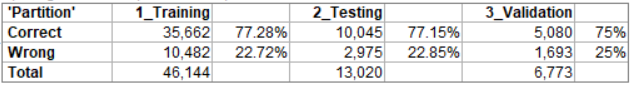
\includegraphics[width=0.9\textwidth]{KNN_analysis.PNG}
                \caption{Analiza modela k najbližih suseda - SPSS}
                \label{fig:knn}
            \end{figure}
            
\subsection{Python}

Primena KNN algoritma je opisana u fajlu \textit{KNN.py}. Veličina trening skupa je postavljena na 95\% i izvršena je stratifikacija. 

\lstinputlisting[language=Python, caption={Najbliži susedi},frame=single, label=knn]{KNN.py}

Najbolji rezultati dobijaju se za k = 9, Euklidsko rastojanje i kada svi susedi imaju podjednak uticaj, što se vidi u tabeli \ref{tab:knn}.
\begin{table}[ht!]
            \begin{center}
            \caption{Analiza modela k najbližih suseda - Python}
            \label{tab:knn}
            \begin{tabular}{c|c|c|c} \hline
            & \textbf{preciznost} & \textbf{f1-skor} & \textbf{tačnost}\\ \hline
            \textbf{LUNG} & 72.00\% & 74.00\% & 68.51\%\\ \hline
            \textbf{HAEMATOPOIETIC} & 63.00\% & 60.00\% & 68.51\%\\ \hline
            \end{tabular}
            \end{center}
        \end{table}

\section{Neuronske mreže}
\label{sec:neuron}

Podaci koji se nalaze u \textit{final\_implicit.xlsx} će biti obrađeni metodom neuronskih mreža u SPSS Modeleru i programskom jeziku Python.

\subsection{SPSS Modeler}

U fajlu \textit{Neurone.str} učitavamo podatke i povezujemo ih sa čvorom \textit{Partition}, koji deli podatke na isti način kao u poglavlju \ref{sec:drveta}. Model se generiše pokretanjem čvora \textit{Neural Net}, povezanim sa čvorom \textit{Partition}. Za cilj je odabrano kreiranje novog višeslojnog modela.

Kreirani model ima 1 skriveni sloj, kao što se vidi na slici \ref{fig:neurone} i razvijao se do trenutka kada više nije bilo moguće smanjiti grešku. Analiza modela prikazana je na slici \ref{fig:neurone_an}.
\begin{figure}[ht!]
                \centering
                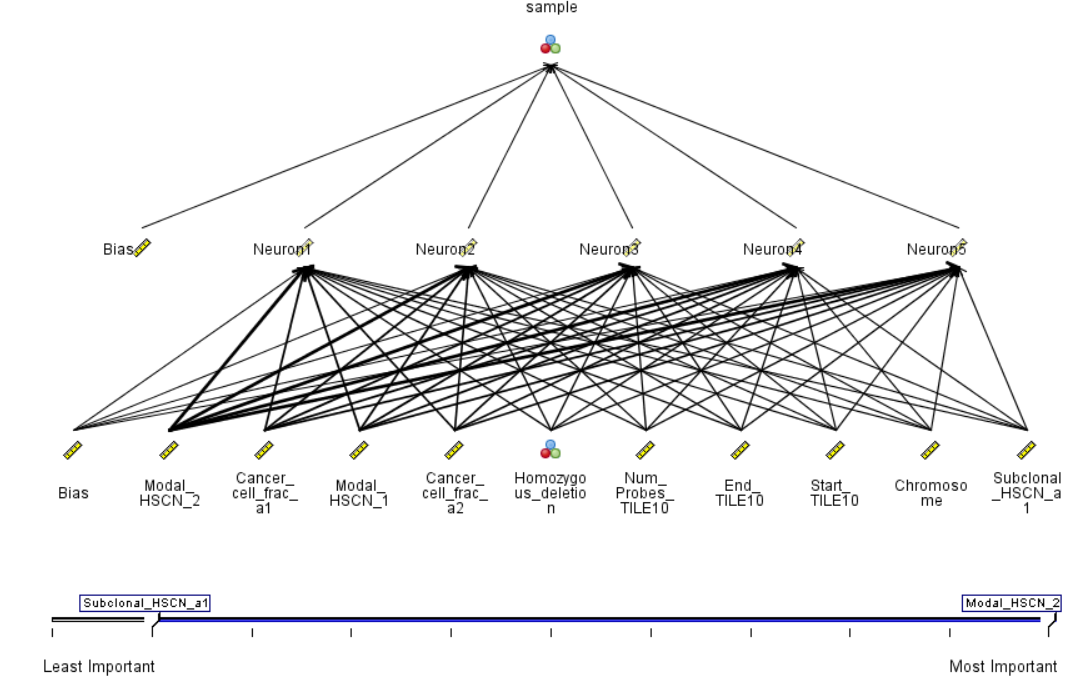
\includegraphics[width=0.9\textwidth]{Neural_model.PNG}
                \caption{Neuronska mreža}
                \label{fig:neurone}
            \end{figure}
            
            \begin{figure}[ht!]
                \centering
                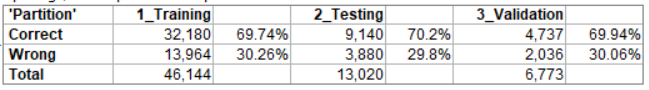
\includegraphics[width=0.9\textwidth]{Neural_analysis.PNG}
                \caption{Analiza modela neuronske mreže - SPSS}
                \label{fig:neurone_an}
            \end{figure}

\subsection{Python}

Ovaj metod je primenjen na podatke u fajlu \textit{final\_implicit.xlsx}, a opisan je u \textit{MLP.py} fajlu, čiji je jedan deo prikazan u Listingu. Nad podacima je izvršena strafifikacija i za trening skup uzeto je 70\% podataka.


\lstinputlisting[language=Python, caption={Neuronske mreže},frame=single, label=MLP]{MLP.py}

Izvršeno je 47 iteracija i to sa 4 sloja. Analiza modela je predstavljena u tabeli
\begin{table}[ht!]
            \begin{center}
            \caption{Analiza MLP modela - Python}
            \label{tab:knn}
            \begin{tabular}{c|c|c|c} \hline
            & \textbf{preciznost} & \textbf{f1-skor} & \textbf{tačnost}\\ \hline
            \textbf{LUNG} & 71.00\% & 76.00\% & 69.74\%\\ \hline
            \textbf{HAEMATOPOIETIC} & 67.00\% & 59.00\% & 69.74\%\\ \hline
            \end{tabular}
            \end{center}
        \end{table}

\section{Metod potpornih vektora}
\label{sec:SVM}

Ovaj metod je primenjen na podatke u fajlu \textit{final\_implicit.xlsx}, a opisan je u \textit{SVM.str} fajlu u kojem najpre učitavamo podatke, a zatim na njima primenjujemo PCA modeliranje koristeći \textit{PCA} čvor, kako bismo odabrali 5 najznačajnijih komponenti i smanjili skup atributa sa kojima se radi. Zatim se vrši podela podataka na trening, test i validacioni skup, nakon čega se pravi model potpornih vektora pomoću čvora \textit{SVM}. Analiza dobijenog modela predstavljena je na slici \ref{fig:svm_an}.

\begin{figure}[ht!]
                \centering
                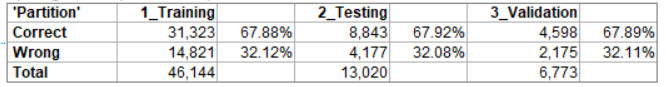
\includegraphics[width=0.9\textwidth]{SVM_analysis.PNG}
                \caption{Analiza modela potpornih vektora}
                \label{fig:svm_an}
            \end{figure}
            
\newpage

\section{Gausova klasifikacija}
\label{sec:gaus}

Ovaj metod je primenjen na podatke u fajlu \textit{final\_implicit.xlsx}, a opisan je u \textit{Gaussian.py} fajlu, čiji je jedan deo prikazan u Listingu. Nad podacima je izvršena strafifikacija i za trening skup uzeto je 70\% podataka.

Analiza podataka prikazana je u tabeli
\begin{table}[ht!]
            \begin{center}
            \caption{Analiza modela dobijenog Gausovom klasifikacijom}
            \label{tab:knn}
            \begin{tabular}{c|c|c|c} \hline
            & \textbf{preciznost} & \textbf{f1-skor} & \textbf{tačnost}\\ \hline
            \textbf{LUNG} & 58.00\% & 60.00\% & 65.74\%\\ \hline
            \textbf{HAEMATOPOIETIC} & 72.00\% & 70.00\% & 65.74\%\\ \hline
            \end{tabular}
            \end{center}
        \end{table}

\lstinputlisting[language=Python, caption={Gausova klasifikacija},frame=single, label=gaus]{Gaussian.py}

\newpage

\section{Zaključak}
\label{sec:Zakljucak}

Kako bi algoritmi klasifikacije bili u stanju da daju što preciznije rezultate, neophodno je prethodno ih pripremiti za klasifikaciju. Utvrđeno je da se nad datim skupom podataka najbolji rezultati postižu prilikom rada sa dve klase sa najvećim brojem instanci.  Dodatno, potrebno je izvršiti grupisanje nad instancama koje imaju veliku razliku između minimalne i maksimalne vrednosti.

S obzirom na to da početak i kraj segmenta baznih parova na određenom hromozomu definiše njima odgovarajuću grupu gena, očekivano je da su samo te iste informacije dovoljne da se utvrdi koje je kontaminirano tkivo u pitanju. Međutim, utvrđeno je da algoritmi klasifikacije nisu u stanju da kvalitetno razluče koje tkivo je obolelo samo na osnovu datih podataka. Razlog leži u činjenici da različite vrste kancera imaju  mutirane iste gene, te se zajedno pojavljuju u organizmu. Jedan od najboljih primera su rak dojke i jajnika: pacijenti sa rakom dojke imaju mutirane gene bitne za normalno funkcionisanje jajnika i obrnuto. Međutim, njihove kancerogene ćelije poseduju različite stope duplikacija i delecija, kao i SNP satelita, što olakšava njihovo razlikovanje.

Prilikom ovog istraživanja, najbolji rezultati postignuti su primenom algoritma k najbližih suseda u SPSS Modeleru - utvrđena tačnosti je 75\%. Najlošiji rezultati dobijeni su primenom Gausove klasifikacije - utvrđena tačnost je 65\%.

Konačan odgovr na pitanje da li je istraživanje uspelo ne postoji, samim tim što zavisi iz kog se ugla problem i rešenje posmatraju:  ako se uzme u obzir da se od tačnosti predviđanja koja iznosi 0.5\% došlo do tačnosti koja iznosi , odgovor je \textit{da}; ako se posmatra početni skup podataka, koji sadrži veliki broj klasa, odgovor je \textit{ne}; ako se rezultat istraživanja koristi u naučne svrhe gde je potrebna preciznost po klasi veća od 90\%, odgovor je \textit{ne}; ako se rezultat istraživanja koristi radi upoznavanja sa zakonitostima koje vladaju među sekvenciranim podacima i uopšteno osobinama kancerogenih tkiva, onda je odgovor \textit{da}.

\newpage

\addcontentsline{toc}{section}{Literatura}
\appendix
\bibliography{literatura} 
\bibliographystyle{plain}

\end{document}